\documentclass{article}
\usepackage{amsmath}
\usepackage{titlesec}
\usepackage{graphicx}
\usepackage[margin=1in]{geometry}
\usepackage{hyperref}
\usepackage{float}

% Title, date, and author
\title{Exercise 6}
\author{Your Name, Collaborator's Name}
\date{\today}

\titleformat{\section}
  {\normalfont\normalsize\bfseries} % Format: font style, size, and weight
  {\thesection}{1em} % Label format and spacing
  {}
  \renewcommand{\thesubsection}{\thesection.\alph{subsection}}

\titleformat{\subsection}
  {\normalfont\small\bfseries} % Format: font style, size, and weight
  {\thesubsection}{1em} % Label format and spacing
  {}
\titleformat{\subsubsection}
  {\normalfont\small\bfseries} % Format: font style, size, and weight
  {\thesubsubsection}{1em} % Label format and spacing
  {}

\begin{document}
\begin{titlepage}
    \centering
    \vspace*{1in}
    
    {\Huge\bfseries Exercise 6\par}
    \vspace{1.5cm}
    {\Large \today\par}
    \vspace{1.5cm}
    {\Large\itshape Antonio Pampalone 23586519 \\ Giuseppe Pisante 23610012\\ Martina Raffaelli 23616907 \par}
    
    \vfill
    
\includegraphics[width=0.3\textwidth]{FAU-Logo.png}\par\vspace{1cm} % Adjust the width as needed
   
\end{titlepage}

\newpage
\small

\section{Finite-difference method on a non-uniform grip}

\subsection{Transformation from from physical space into computational space}
Using the chain rule, the first derivative of \(\Phi\) with respect to \(x\) is given by:

\[
\frac{d\Phi}{dx} = \frac{d\Phi}{d\xi} \cdot \frac{d\xi}{dx}
\]
Since we assume that \(\xi\) is the computational space where grid points are equally spaced, we express \( d\xi/dx \) in terms of \( x \):

\[
\frac{d\xi}{dx} = \frac{1}{\frac{dx}{d\xi}}
\]
Substituting this into the previous equation:

\[
\frac{d\Phi}{dx} = \frac{d\Phi}{d\xi} \cdot \frac{1}{\frac{dx}{d\xi}}
\]
Thus, we obtain the compact form:

\begin{equation}
\frac{d\Phi}{dx} = \frac{\frac{d\Phi}{d\xi}}{\frac{dx}{d\xi}}.
\end{equation}
The second derivative is defined as:

\[
\frac{d^2\Phi}{dx^2} = \frac{d}{dx} \left( \frac{d\Phi}{dx} \right).
\]
Substituting \(\frac{d\Phi}{dx} = \frac{\frac{d\Phi}{d\xi}}{\frac{dx}{d\xi}}\):

\[
\frac{d^2\Phi}{dx^2} = \frac{d}{dx} \left( \frac{\frac{d\Phi}{d\xi}}{\frac{dx}{d\xi}} \right).
\]
Using the chain rule:

\[
\frac{d^2\Phi}{dx^2} = \frac{d}{d\xi} \left( \frac{\frac{d\Phi}{d\xi}}{\frac{dx}{d\xi}} \right) \cdot \frac{d\xi}{dx}.
\]
Again, substituting \( \frac{d\xi}{dx} = \frac{1}{\frac{dx}{d\xi}} \), we get:

\[
\frac{d^2\Phi}{dx^2} = \frac{\frac{d}{d\xi} \left( \frac{\frac{d\Phi}{d\xi}}{\frac{dx}{d\xi}} \right)}{\frac{dx}{d\xi}}.
\]
Now, applying the quotient rule to differentiate:

\[
\frac{d}{d\xi} \left( \frac{\frac{d\Phi}{d\xi}}{\frac{dx}{d\xi}} \right) =
\frac{\frac{d^2\Phi}{d\xi^2} \cdot \frac{dx}{d\xi} - \frac{d\Phi}{d\xi} \cdot \frac{d^2x}{d\xi^2}}{\left( \frac{dx}{d\xi} \right)^2}.
\]
Substituting this result:

\[
\frac{d^2\Phi}{dx^2} = \frac{\frac{\frac{d^2\Phi}{d\xi^2} \cdot \frac{dx}{d\xi} - \frac{d\Phi}{d\xi} \cdot \frac{d^2x}{d\xi^2}}{\left( \frac{dx}{d\xi} \right)^2}}{\frac{dx}{d\xi}}.
\]
Multiplying by \( \frac{1}{\frac{dx}{d\xi}} \), we obtain:

\begin{equation}
\frac{d^2\Phi}{dx^2} = \frac{\frac{d^2\Phi}{d\xi^2}}{\left( \frac{dx}{d\xi} \right)^2} - \frac{\frac{d^2x}{d\xi^2} \cdot \frac{d\Phi}{dx}}{\left( \frac{dx}{d\xi} \right)^2}.
\end{equation}
These expressions can be used to transform differential equations from physical space into computational space.

\subsection{Non-uniform grid}
Non-uniform grids are often used because they allow for adaptive resolution in areas where higher accuracy or detail is needed 
such as boundary layers, shocks, or vortices without increasing computational cost significantly across the entire domain. 
By refining the grid only where necessary, non-uniform grids reduce the number of total grid points, saving memory and computational time.
Furthermore non-uniform grids are better suited for domains with irregular or complex geometries since the grid can better conform to 
the shape of the domain, improving accuracy in boundary condition enforcement.

\subsection{Central finite-difference approximation on an non-equispaced grid}
To derive central finite-difference approximations for the first and second derivatives in the computational space \(\xi\) with second-order 
accuracy, we start from equation (1) and (2). For the first derivative we start computing the central finite-difference approximation for the term:

\[
\frac{d\Phi}{d\xi} \approx \frac{\Phi_{i+1} - \Phi_{i-1}}{2\Delta \xi},
\]
where \(\Delta \xi = 1\). Here \(\frac{dx}{d\xi}\) is computed based on the grid points \(x_i\).

\[
\frac{dx}{d\xi} \approx \frac{x_{i+1} - x_{i-1}}{2\Delta \xi}.
\]
Substituting into the equation (1) we get:

\begin{equation}
\frac{d\Phi}{dx} \approx \frac{\frac{\Phi_{i+1} - \Phi_{i-1}}{2}}{\frac{x_{i+1} - x_{i-1}}{2}} = \frac{\Phi_{i+1} - \Phi_{i-1}}{x_{i+1} - x_{i-1}}.
\end{equation}
Similary, to derive an approximation for the second derivative, we start computing the central finite-difference approximation for the term:

\[
\frac{d^2\Phi}{d\xi^2} \approx \frac{\Phi_{i+1} - 2\Phi_i + \Phi_{i-1}}{\Delta \xi^2}.
\]
where \(\Delta \xi = 1\). Here \(\frac{d^2x}{d\xi^2}\) is computed based on the grid points \(x_i\).

\[
\frac{d^2x}{d\xi^2} \approx x_{i+1} - 2x_i + x_{i-1}.
\]
Substituting into the equation (2) we get:

\begin{equation}
\frac{d^2\Phi}{dx^2} \approx \frac{\Phi_{i+1} - 2\Phi_i + \Phi_{i-1}}{\left(\frac{x_{i+1} - x_{i-1}}{2}\right)^2} - \frac{\left(x_{i+1} - 2x_i + x_{i-1}\right) \cdot \frac{\Phi_{i+1} - \Phi_{i-1}}{x_{i+1} - x_{i-1}}}{\left(\frac{x_{i+1} - x_{i-1}}{2}\right)^2}.
\end{equation}

\subsection{Discretized steady one-dimensional advection-diffusion equation}
Using central finite-difference approximations for the first and second derivatives on a non-uniform grid, we want to discretize 
the steady one-dimensional advection-diffusion equation. Substituting equation (3) and (4) into the advection-diffusion equation leads to:
\[
\frac{\Phi_{i+1} - \Phi_{i-1}}{x_{i+1} - x_{i-1}} = \frac{1}{\text{Pe}} \left[ \frac{\Phi_{i+1} - 2\Phi_i + \Phi_{i-1}}{\left(\frac{x_{i+1} - x_{i-1}}{2}\right)^2} - \frac{\left(x_{i+1} - 2x_i + x_{i-1}\right) \cdot \frac{\Phi_{i+1} - \Phi_{i-1}}{x_{i+1} - x_{i-1}}}{\left(\frac{x_{i+1} - x_{i-1}}{2}\right)^2} \right].
\]
Rearranging the above equation, the discretized equation for an interior point \(i\) becomes:

\[
a_{i-1} \Phi_{i-1} + b_i \Phi_i + c_{i+1} \Phi_{i+1} = 0,
\]
where:
\[
a_{i-1} = \frac{-1}{\Delta x_i} + \frac{1}{\text{Pe}} \left( \frac{1}{\Delta x_i^2} - \frac{x_{i+1} - 2x_i + x_{i-1}}{\Delta x_i^2} \right),
\]
\[
b_i = \frac{2}{\text{Pe} \cdot \Delta x_i^2},
\]
\[
c_{i+1} = \frac{1}{\Delta x_i} + \frac{1}{\text{Pe}} \left( \frac{1}{\Delta x_i^2} + \frac{x_{i+1} - 2x_i + x_{i-1}}{\Delta x_i^2} \right).
\]
Here, \(\Delta x_i = x_{i+1} - x_{i-1}\).
The discretized system can be expressed in matrix form as:
\[
\mathbf{A} \boldsymbol{\Phi} = \mathbf{b},
\]
where:
\begin{itemize}
    \item \(\mathbf{A}\) is an \(N \times N\) sparse coefficient matrix,
    \item \(\boldsymbol{\Phi} = [\Phi_1, \Phi_2, \dots, \Phi_N]^T\) is the vector of unknowns,
    \item \(\mathbf{b}\) is the right-hand side vector, accounting for boundary conditions.
\end{itemize}
For \(N\) grid points, the coefficient matrix \(\mathbf{A}\) is tridiagonal for interior points:

\[
\mathbf{A} =
\begin{bmatrix}
b_1 & c_2 & 0 & \cdots & 0 \\
a_2 & b_2 & c_3 & \cdots & 0 \\
0 & a_3 & b_3 & \cdots & 0 \\
\vdots & \vdots & \vdots & \ddots & c_{N-1} \\
0 & 0 & 0 & a_{N} & b_{N}
\end{bmatrix}.
\]

\section{Implementation of Task 6.1}
The implementation of Task 6.1 can be found in the GitHub repository at the following link: \url{https://github.com/GiuseppePisante/CFD.git}. 
The code is located in the \texttt{exercise6} folder. The figure illustrates the numerical solution of the advection-diffusion equation 
using the finite difference method for different grid resolutions and using a non-uniform discretization. 

\begin{figure}[h!]
  \centering
  \begin{minipage}{0.32\textwidth}
      \centering
      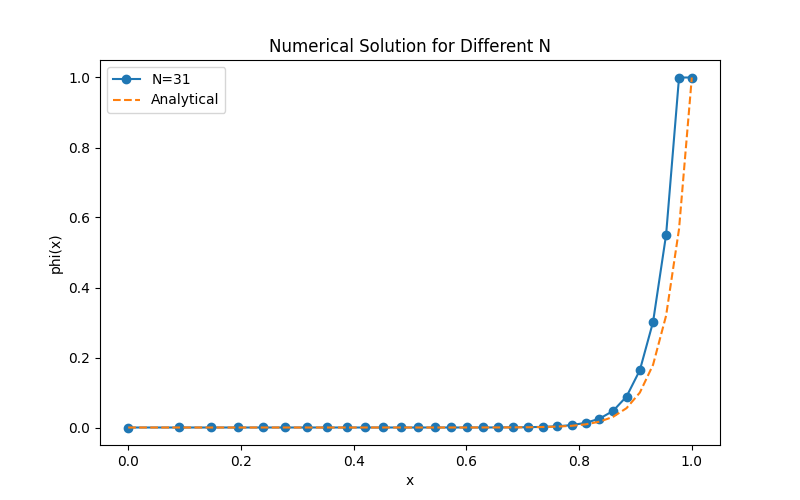
\includegraphics[width=\textwidth]{FDM_32.png}
      \label{fig:32}
  \end{minipage} \hfill
  \begin{minipage}{0.32\textwidth}
      \centering
      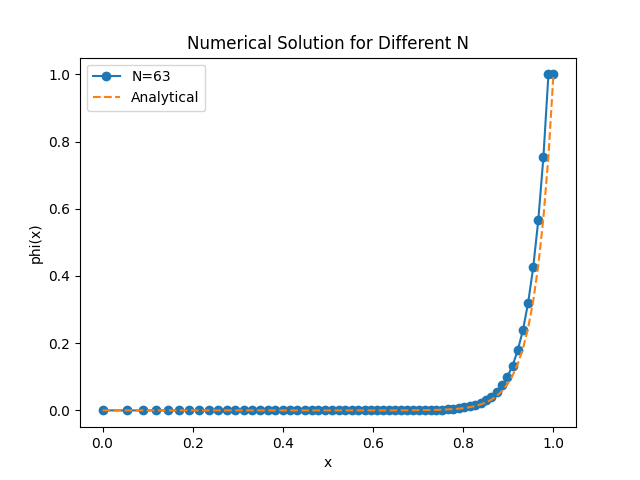
\includegraphics[width=\textwidth]{FDM_64.png}
      \label{fig:64}
  \end{minipage} \hfill
  \begin{minipage}{0.32\textwidth}
      \centering
      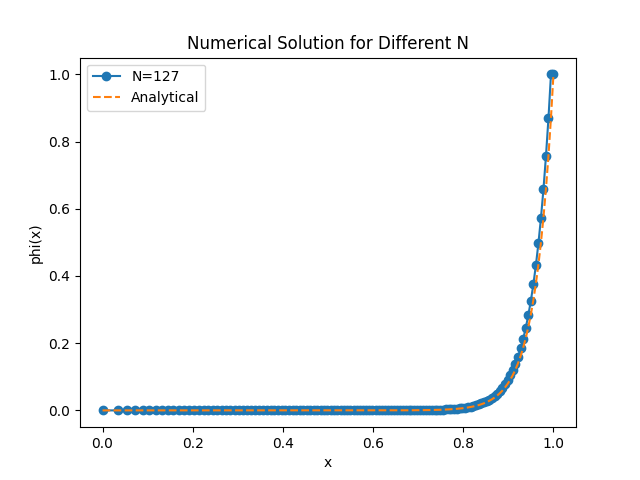
\includegraphics[width=\textwidth]{FDM_128.png}
      \label{fig:128}
  \end{minipage}
  \caption{Comparison of numerical solutions of the advection-diffusion equation with different inner points.}
  \label{fig:comparison}
\end{figure}

\subsection{Error Analysis and Order of Accuracy}

The numerical results are compared with the analytical solution to evaluate accuracy. The computed L1 and L2 errors show a clear trend of 
decreasing as the grid is refined. By doubling the number of grid points from N = 32 to N = 64 and then to N = 128, the errors decrease, 
confirming that the numerical method is consistent and convergent. The computed errors for different grid resolutions are as follows:

\begin{itemize}
    \item \textbf{L1 Errors:}
    \begin{itemize}
        \item $N = 32$: \quad $0.03057$
        \item $N = 64$: \quad $0.01495$
        \item $N = 128$:\quad $0.00751$
    \end{itemize}
    
    \item \textbf{L2 Errors:}
    \begin{itemize}
        \item $N = 32$: \quad $0.09336$
        \item $N = 64$: \quad $0.04549$
        \item $N = 128$:\quad $0.02278$
    \end{itemize}
\end{itemize}
The order of accuracy is computed as follows:

\begin{itemize}
    \item \textbf{Estimated Order of Accuracy (L1):}
    \begin{itemize}
        \item From $N = 32$ to $N = 64$: \quad $1.032$
        \item From $N = 64$ to $N = 128$:\quad $0.994$
    \end{itemize}
    
    \item \textbf{Estimated Order of Accuracy (L2):}
    \begin{itemize}
        \item From $N = 32$ to $N = 64$: \quad $1.037$
        \item From $N = 64$ to $N = 128$:\quad $0.997$
    \end{itemize}
\end{itemize}
A comparison between the L1 and L2 norms highlights that the two metrics behave similarly, with the L2 norm generally being 
slightly larger than the L1 norm. This is due to the fact that the L2 norm squares the error before averaging, making it more 
sensitive to localized discrepancies in the numerical solution. Overall, the results confirm that the chosen numerical method 
is consistent and convergent, with a convergence rate close to first order. 

\begin{figure}[h!]
  \centering
  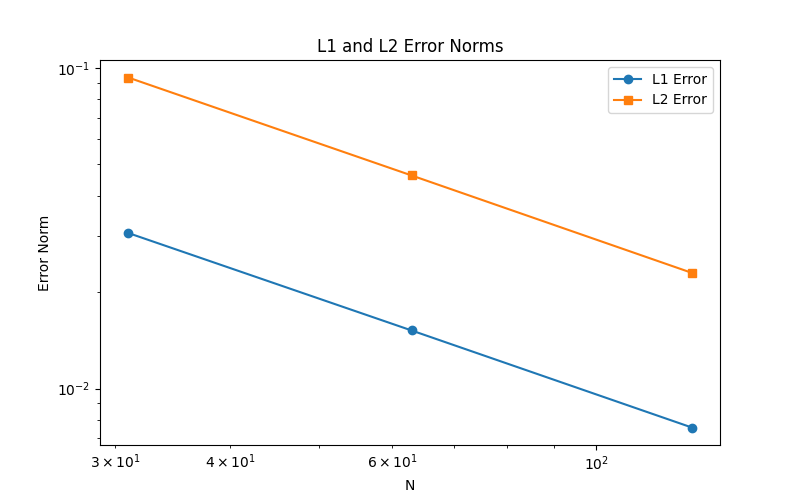
\includegraphics[width=0.5\textwidth]{FDM_Error.png}
  \caption{L1 and L2 norms}
\end{figure}

\subsection{Check of conservation property}

To verify whether a finite-difference implementation is conservative, we need to show the following two conditions that the volume integral 
of the equation must be equal to the difference of the flux at the boundaries and that the difference in flux between the two boundaries must 
be zero. The general conservation law is given by the differential equation:

\begin{equation}
    \frac{\partial u}{\partial t} + \frac{\partial f}{\partial x} = 0,
\end{equation}
Integrating this equation over a control volume $[a, b]$:

\begin{equation}
    \int_{a}^{b} \frac{\partial u}{\partial t} dx + \int_{a}^{b} \frac{\partial f}{\partial x} dx = 0.
\end{equation}
Applying the fundamental theorem of calculus to the flux term:

\begin{equation}
    \frac{d}{dt} \int_{a}^{b} u \, dx + \left[ f(b) - f(a) \right] = 0.
\end{equation}
This equation states that the rate of change of the total quantity $u$ inside the volume is balanced by the difference in flux at the two boundaries.
For a numerical scheme to be conservative, the flux leaving one control volume must equal the flux entering the next. In a discretized form, this can be written as:

\begin{equation}
    f_{i+\frac{1}{2}} - f_{i-\frac{1}{2}} = 0.
\end{equation}
Summing over all grid cells, the internal flux terms cancel, leaving only the boundary fluxes. If the boundary fluxes are handled correctly, 
the net flux difference should be zero, ensuring conservation.


\section{Finite-volume method on a non-uniform grip}

\subsection{Integral form of the convection-diffusion equation}

To reformulate the general form of the steady-state advection-diffusion equation in integral form we need to integrate the equation
over a control volume \( V \):

\[
\int_V \mathbf{u} \cdot \nabla \Phi \, dV = \int_V \frac{1}{Pe} \nabla^2 \Phi \, dV
\]
Applying the divergence theorem to both terms we get:

\[
\oint_A (\mathbf{u} \Phi) \cdot \mathbf{n} \, dA = \oint_A \left( \frac{1}{Pe} \nabla \Phi \right) \cdot \mathbf{n} \, dA
\]
Where the left-hand side represents the net convective flux of \( \Phi \) across the control volume surface 
and the right-hand side represents the net diffusive flux of \( \Phi \) across the control volume surface.

\subsection{Approximation for the convective and diffusion terms}

For convection, we approximate \( \Phi \) at the control volume faces using linear interpolation:

\[
\Phi_{i+\frac{1}{2}} = w \Phi_i + (1 - w) \Phi_{i+1}
\]

\[
\Phi_{i-\frac{1}{2}} = w' \Phi_{i-1} + (1-w') \Phi_{i} 
\]
where \( w \) and \( w' \) are the interpolation weight depending on the grid spacing:

\[
w = \frac{x_{i+1} - x_i}{x_{i+1} - x_{i+\frac{1}{2}}}
\]

\[
w' = \frac{x_i - x_{i-\frac{1}{2}}}{x_i - x_{i-1}}
\]
Thus, the convective flux at \( x_{i+\frac{1}{2}} \) is:

\[
F_{c, i+\frac{1}{2}} = u_{i+\frac{1}{2}} \Phi_{i+\frac{1}{2}}
\]
Similarly, at \( x_{i-\frac{1}{2}} \):

\[
F_{c, i-\frac{1}{2}} = u_{i-\frac{1}{2}} \Phi_{i-\frac{1}{2}}
\]
For diffusion, we approximate the derivative at the control volume faces using a central difference scheme:

\[
\left( \frac{d\Phi}{dx} \right)_{i+\frac{1}{2}} \approx \frac{\Phi_{i+1} - \Phi_i}{x_{i+1} - x_i}
\]

\[
\left( \frac{d\Phi}{dx} \right)_{i-\frac{1}{2}} \approx \frac{\Phi_i - \Phi_{i-1}}{x_i - x_{i-1}}
\]
Thus, the diffusive flux at \( x_{i+\frac{1}{2}} \) is:

\[
F_{d, i+\frac{1}{2}} = - \frac{1}{Pe} \frac{\Phi_{i+1} - \Phi_i}{x_{i+1} - x_i}
\]
Similarly, at \( x_{i-\frac{1}{2}} \):

\[
F_{d, i-\frac{1}{2}} = - \frac{1}{Pe} \frac{\Phi_i - \Phi_{i-1}}{x_i - x_{i-1}}
\]
The linear interpolation for \( \Phi_{i+\frac{1}{2}} \) introduces first-order accuracy in the convection term. The central difference scheme 
for diffusion is second-order accurate but the overall accuracy of the discretization is first order due to the convection term.

\subsection{Discretization and Matrix Form Representation of the Advection-Diffusion Equation}

The general discrete equation for an interior node \(i\) is:

\[
F_{c, i+\frac{1}{2}} - F_{c, i-\frac{1}{2}} + F_{d, i+\frac{1}{2}} - F_{d, i-\frac{1}{2}} = 0
\]
Expanding:

\[
u_{i+\frac{1}{2}} \Phi_{i+\frac{1}{2}} - u_{i-\frac{1}{2}} \Phi_{i-\frac{1}{2}} - \frac{1}{Pe} \frac{\Phi_{i+1} - \Phi_i}{x_{i+1} - x_i} + \frac{1}{Pe} \frac{\Phi_i - \Phi_{i-1}}{x_i - x_{i-1}} = 0
\]
Substituting both flux terms and simplifying, the general discrete equation for an interior node \(i\) is:

\[
a_{i-1} \Phi_{i-1} + a_i \Phi_i + a_{i+1} \Phi_{i+1} = 0
\]
where the coefficients are:

\[
a_{i-1} = -\frac{1}{Pe} \frac{1}{x_i - x_{i-1}} - u_{i-\frac{1}{2}} w'
\]
\[
a_i = \frac{1}{Pe} \left( \frac{1}{x_i - x_{i-1}} + \frac{1}{x_{i+1} - x_i} \right) + u_{i+\frac{1}{2}} w - u_{i-\frac{1}{2}} (1 - w')
\]
\[
a_{i+1} = -\frac{1}{Pe} \frac{1}{x_{i+1} - x_i} - u_{i+\frac{1}{2}} (1 - w)
\]
For an \(N\)-point grid, we obtain a system of equations in matrix form:

\[
A \Phi = b
\]
where:
\begin{itemize}
    \item \(\mathbf{A}\) is an \(N \times N\) sparse coefficient matrix,
    \item \(\boldsymbol{\Phi} = [\Phi_1, \Phi_2, \dots, \Phi_N]^T\) is the vector of unknowns,
    \item \(\mathbf{b}\) is the right-hand side vector, accounting for boundary conditions.
\end{itemize}
For \(N\) grid points, the coefficient matrix \(\mathbf{A}\) is tridiagonal for interior points:

\[
\begin{bmatrix}
a_1 & a_2 & 0 & 0 & \dots & 0 \\
a_{-1} & a_1 & a_2 & 0 & \dots & 0 \\
0 & a_{-1} & a_1 & a_2 & \dots & 0 \\
\vdots & \vdots & \vdots & \vdots & \ddots & \vdots \\
0 & 0 & 0 & a_{-1} & a_1 & a_2
\end{bmatrix}
\begin{bmatrix}
\Phi_1 \\
\Phi_2 \\
\Phi_3 \\
\vdots \\
\Phi_{N-1}
\end{bmatrix}
=
\begin{bmatrix}
b_1 \\
b_2 \\
b_3 \\
\vdots \\
b_{N-1}
\end{bmatrix}
\]

\section{Implementation of Task 6.2}
The implementation of Task 6.2 can be found in the GitHub repository at the following link: \url{https://github.com/GiuseppePisante/CFD.git}. 
The code is located in the \texttt{exercise6} folder. The figure illustrates the numerical solution of the advection-diffusion equation using 
the finite volume method for different grid resolutions and using a non-uniform discretization. 

\begin{figure}[h!]
  \centering
  \begin{minipage}{0.32\textwidth}
      \centering
      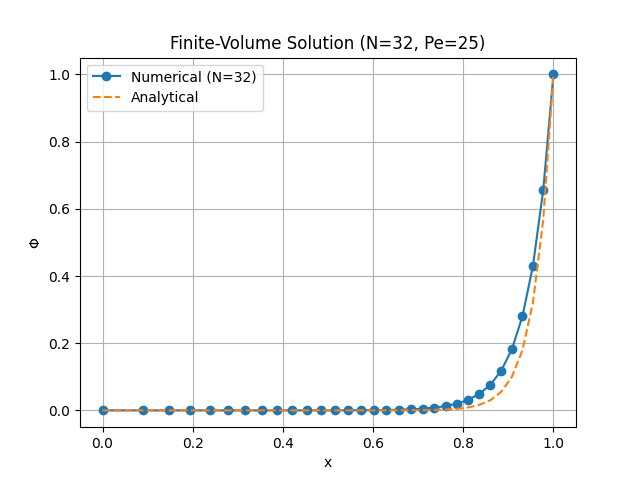
\includegraphics[width=\textwidth]{FVM_32.png}
      \label{fig:32}
  \end{minipage} \hfill
  \begin{minipage}{0.32\textwidth}
      \centering
      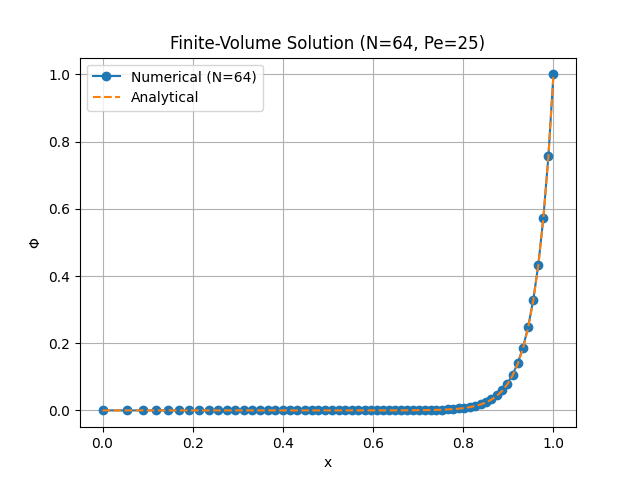
\includegraphics[width=\textwidth]{FVM_64.png}
      \label{fig:64}
  \end{minipage} \hfill
  \begin{minipage}{0.32\textwidth}
      \centering
      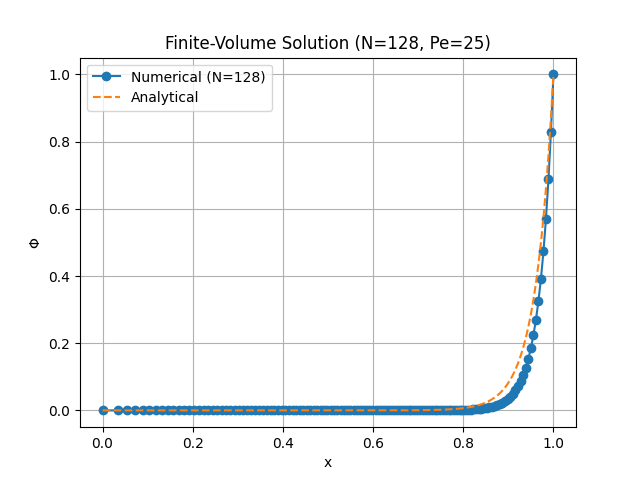
\includegraphics[width=\textwidth]{FVM_128.png}
      \label{fig:128}
  \end{minipage}
  \caption{Comparison of numerical solutions of the advection-diffusion equation with different inner points.}
  \label{fig:comparison}
\end{figure}








\begin{thebibliography}{9}
    \bibitem{GitHubRepo}
    \textit{CFD Repository},\\
    Available at: \url{https://github.com/GiuseppePisante/CFD.git}
    
    \bibitem{GitHubCopilot}
    \textit{GitHub Copilot},\\
    GitHub. Available at: \url{https://github.com/features/copilot}
  \end{thebibliography}
  
  \end{document}